\documentclass[10pt]{article}

\topmargin      = -.25in
\textwidth      = 6.5in
\textheight     = 8.5in
\oddsidemargin  = 0in
\evensidemargin = 0in

\usepackage[inline]{enumitem}
\usepackage{tikz}
\usepackage{amsmath}
\usetikzlibrary{positioning}
\usepackage{hyperref}
\usepackage{listings}

\def\hwid{4}
\def\course{{\Large CS 161: Fundamentals of Artificial Intelligence}}
\def\quarter{Spring 2023}
\def\hw{Assignment 4}
\def\due{11:30pm, Tuesday, MAY 2}


% some macros

\def\iff{if\mbox{}f }

\def\entails{\models}
\def\implies{\Rightarrow}
\def\negg(#1){\overline{#1}}

\def\pr{{\sf Pr}}
\def\true{{\sf true}}
\def\false{{\sf false}}
\def\dsep{{\sf dsep}}
 
\def\X{{\bf X}}
\def\x{{\bf x}}
\def\Q{{\bf Q}}
\def\q{{\bf q}}
\def\R{{\bf R}}
\def\r{{\bf r}}

\newtheorem{example}{Example}



\begin{document}

% HEADER
\noindent\rule{\textwidth}{.5mm}
\begin{center} \course\\
\vspace{1mm}Prof. Darwiche \\ 
\vspace{4mm}{\quarter\ -- \hw\ -- Due \due}
\end{center}
\noindent \rule{\textwidth}{.5mm}
\vspace{2mm}

% BODY


In this assignment you will write a Python program that converts graph coloring problems into SAT problems and use a SAT solver to solve them. The graph coloring problem concerns if there exists an assignment of colors to nodes of a graph such that no two adjacent nodes are of the same color. Your task consists of two steps:

\begin{enumerate}
    \item (70 pts) Convert a graph coloring instance into a boolean formula $\Delta$ in {\em Conjunctive Normal Form} (CNF).
    \item (30 pts) Decide if $\Delta$ is satisfiable by invoking the RSat solver (http://reasoning.cs.ucla.edu/rsat/). 
\end{enumerate}

We have broken the task into multiple functions and provided you with some basic code for file I/O and for gluing all the functions together (see {\bf hw4\_skeleton.py}).

% Extra credits (20 pts): you can build your own SAT solver by treating SAT as a Constraint Satisfication Problem (CSP) and solving it using backtracking search. You can then compare the solution of your solver to that of the RSAT solver.

\section{CNF}\label{sec:CNF}
A boolean sentence $\Delta$ is in CNF if it is a conjunction of {\em clauses}, where a clause is a disjunction
of literals (a literal is a variable or its negation). 

\begin{example}
The following sentence $\Delta$ is a CNF defined over three Boolean variables $X, Y, Z$.

\[
    \Delta = (X \lor \neg Y \lor Z) \land \neg X \land (\neg Y \lor \neg Z)
\]
It has three clauses: $X \lor \neg Y \lor Z, \neg X, \neg Y \lor \neg Z$ and five literals: $X, \neg X, \neg Y, Z, \neg Z$.
\end{example}
In this assignment, each Boolean variable is represented by a positive integer (variable index). As a result, a positive integer is used for a positive literal and a negative integer is used for a negative literal. A clause is simply a list containing the literals of the clause. A CNF formula is then simply a list of clauses. For example, if variable $X$ has index 1, variable $Y$ has index 2, and variable $Z$ has index 3, then the clause $X \lor \neg Y \lor Z$ is represented as a list $[1, -2, 3]$, and the above CNF $\Delta$ is then represented as a list of list $[[1, -2, 3],[-1],[-2,-3]]$. Of course, the order of clauses and literals in each clause does not matter.

\section{Convert Graph Coloring to SAT}
Consider a graph $G$ and $k$ possible colors (whose nodes are labeled with their node indices as below). We next show the procedures to construct a CNF from a graph coloring problem.

\begin{figure}[h]
    \centering
    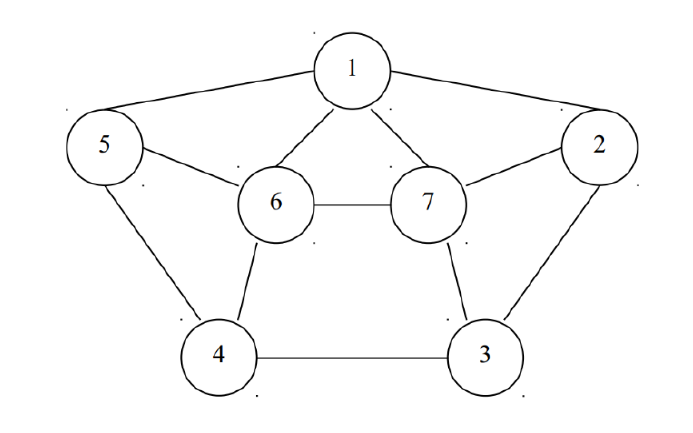
\includegraphics[width=7cm]{graph1.png}
    \caption{Example graph in graph1.txt}
    \label{fig:graph1}
\end{figure}

\begin{enumerate}
    \item For each node $n$ and for each color $c$, create a boolean variable to represent whether node $n$ is assigned color $c$. You will write a function \texttt{node2var(n, c, k)}. This function should return the index of the Boolean variable that represents the condition that node $n$ is assigned color $c$ (with $k$ colors being considered). Use the following conversion convention:
   \[
      \text{variable index}=(n-1)\cdot k+c.
   \]
   \item For each node $n$, add a clause to represent the constraint that a node is assigned {\em at least} one color whose index comes from the set $\{1,2,\ldots,k\}$. You will write a function \texttt{at\_least\_one\_color(n, k)} that takes a node index and returns this clause.
   \item For each node $n$, add a list of clauses to represent the constraint that a node is assigned {\em at most} one color whose index comes from the set $\{1,2,\ldots,k\}$. You will write a function \texttt{at\_most\_one\_color(n, k)} that takes a node index and returns this list of clauses. You will also write a function \texttt{generate\_node\_clauses(n, k)}. This function should return a list of clauses that constrain node $n$ to be colored with {\em exactly} one color from the set $\{1,2,…,k\}$.
   \item For each edge $(m,n)$ in the graph, add a list of clauses to represent the constraint that prohibits two adjacent nodes $m$ and $n$ to be assigned the same color from the set $\{1,2,…,k\}$.  You will write a function \texttt{generate\_edge\_clauses(e, k)}. An (undirected) edge $e$ is simply a tuple of two node indices $m, n$. This function takes an edge {\tt e} and returns this list of clauses.
\end{enumerate}

After finishing all the above parts, you should be able to convert a graph coloring problem into a SAT problem. To do so, call 

\begin{lstlisting}
    graph_coloring_to_sat(graph_fl, sat_fl, k)
\end{lstlisting}

Here, {\tt graph\_fl} is the filename of the input graph file (e.g. ``graph1.txt"). {\tt sat\_fl} is the name of the output file you want the program to write to (e.g. ``graph1.cnf"). k is the number of possible colors being considered in the problem. We provide two example graphs in {\em graph1.txt} and {\em graph2.txt}. FYI, the graph file has the following format:

\begin{itemize}
    \item[-] The first line contains 2 numbers. The first one is the number of vertices in the graph; the second one is the number of edges.
    \item[-] Each subsequent line describes an edge. An edge is represented by two numbers—the node indices of the two nodes linked by the edge.
\end{itemize}

Now that you have the conversion program working, you can convert the graph coloring problem of the graph provided in graph1.txt with $k=3$ and $k=4$ colors into CNFs respectively. Save the generated CNFs with filenames \textbf{ graph1\_3.cnf} and \textbf{ graph1\_4.cnf} respectively and submit them together with your code.

\section{Solve SAT with RSat}
We show previouly how to convert a graph coloring problem into a SAT instance. The generated CNFs are saved in .cnf files. We can now solve the SAT instance with RSat solver.

Download the RSat SAT solver from (http://reasoning.cs.ucla.edu/rsat/). Read the manual carefully. Use RSat to solve the SAT instance obtained above (in .cnf files) and answer the following questions:

\begin{enumerate}
    \item Consider the CNF generated from graph 1 with $k=3$ colors (graph1\_3.cnf). Is this SAT instance satisfiable?
    \item Consider the CNF generated from graph 1 with $k=4$ colors (graph1\_4.cnf). Is this SAT instance satisfiable?
    \item What do the answers of these two SAT instances tell you about the graph coloring problem of the above graph? Can you give a solution (a coloring assignment) to the graph coloring problem of graph 1 based on the results of RSat?
    \item Use a similar approach to solve the graph coloring problem of graph 2 in graph2.txt. What is the minimum number of colors required to properly color this graph?
\end{enumerate}

Write your answers to the above questions in \textbf{report.txt}. The answer should be clear and concise.


% \section{Extra Credits: build your own SAT solver}
% You are encouraged to build your own SAT solver as an alternative to RSat in this section. You can treat a SAT problem as a CSP Problem and solve it using backtracking search while detecting states that violate constraints. {\bf This section is completely optional}.

% Your top-level function should have signature {\tt SAT(clauses, N)} where {\tt clauses} is a list of clauses that represent a CNF $\Delta$ as described in Section \ref{sec:CNF} and N is the number of variables in this CNF. If $\Delta$ is satisfiable, your function should return a list of N integers that represents a model of $\delta$ (i.e. a satisfying assignment), otherwise it should return an empty list. If $\Delta$ has more than one models, you can return any of the models, and the order of literals in the model is arbitrary.  You are encouraged to use techniques discussed in class to improve the performance of backtracking search, such as variable ordering and forward checking in particular.


% \begin{example} 
%     Consider the following CNF with $N=3$ variables. 
%     \[
%         \Delta = (X \lor \neg Y \lor Z) \land \neg X \land (\neg Y \lor \neg Z)
%     \]
%     Suppose variable $X$ has index 1, variable $Y$ has index 2, and variable $Z$ has index 3. We have
%     \begin{itemize}
%         \item clauses = $[[1, -2, 3],[-1],[-2,-3]]$
%         \item $\{X = \false, Y = \false, Z = \true\}$ is a model of this CNF, which can be represented by $[-1, -2, 3]$. This is a valid result to return.
%         \item The order of literals in the model is arbitrary, so $[-2, -1, 3]$ is also a valid result to return.
%         \item $\{X = \false, Y = \false, Z = \false \}$ also satisfies this CNF, so $[-1, -2, -3]$ is also a valid result.
%     \end{itemize}
% \end{example}






\section*{Submission}



\begin{itemize}
  \item Submit all solution files \textbf{on bruinlearn}.
  \item Submit your Python program in a file \textbf{named hw4.py}.
  \item Submit two files \textbf{graph1\_3.cnf} and \textbf{graph1\_4.cnf} that contains the CNF generated from graph1.txt with $k=3$ and $k=4$ colors respectively.
  \item Submit a report named \textbf{report.txt} that contains your solution to the four questions in Section 3.
  \item Your programs should be written in good style. In Python, a comment is any character following a hash character (\#) on a line. Provide an overall comment explaining your solutions. Furthermore, every function should have a header comment explaining precisely what its arguments are, and what value it returns in terms of its arguments. In addition, you should use meaningful variable names.
  \item The physical layout of the code on the page is very important for making python programs readable. Make sure that you use blank lines between functions and indent properly. Programming style will be a consideration in grading the assignment.
  \item You are restricted to using the python built-in functions. All other packages made by \verb|import| (like \verb|numpy|, \verb|queue|, and \verb|collections|) are forbidden.
  \item You may assume that all input to your functions is legal; i.e. you do not need to
validate inputs.
  \item Do not write any additional helper functions for your code unless this is explicitly
allowed. Test functions are OK.
  \item Your function declarations should look \textbf{exactly as specified} in this assignment. Make
sure the functions are spelled correctly, take the correct number of arguments, and
those arguments are in the correct order.
  \item Even if you are not able to implement working versions of these functions, please \textbf{include a correct skeleton} of each. Some of these assignments are auto graded and having missing functions is problematic.
  \item By submitting this homework, you agree to the following honor code.
  
  You are encouraged to work on your own in this class. If you get stuck, you may discuss the problem with up to two other students, \textbf{PROVIDED THAT YOU SUBMIT THEIR NAMES ALONG WITH YOUR ASSIGNMENT. ALL SOLUTIONS MUST BE WRITTEN UP INDEPENDENTLY, HOWEVER}. This means that you should never see another student's solution before submitting your own. You may always discuss any problem with me or the TAs. \textbf{YOU MAY NOT USE OLD SOLUTION SETS UNDER ANY CIRCUMSTANCES}. Making your solutions available to other students, \textbf{EVEN INADVERTENTLY} (e.g., by keeping backups on github), is aiding academic fraud, and will be treated as a violation of this honor code.

  You are expected to subscribe to the highest standards of academic honesty. This means that every idea that is not your own must be explicitly credited to its author. Failure to do this constitutes plagiarism. Plagiarism includes using ideas, code, data, text, or analyses from any other students or individuals, or any sources other than the course notes, without crediting these sources by name. Any verbatim text that comes from another source must appear in quotes with the reference or citation immediately following. Academic dishonesty will not be tolerated in this class. Any student suspected of academic dishonesty will be reported to the Dean of Students. A typical penalty for a first plagiarism offense is suspension for one quarter. A second offense usually results in dismissal from the University of California.
  

\end{itemize}

\end{document}

